
\lchapter{HOG}

% ---------------------------------------
\section{Introduction}

Le descripteur HOG (Histograms of Oriented Gradients) a été présenté en 2005 dans le cadre de la détection de personnes \cite{NavneetHOG}. En quelques mots, l'image est découpée en plusieurs cellules régulières, dans lesquelles on va décrire la forme locale et l'apparence de l'objet avec un histogramme des directions du gradient ou des orientations des contours.

Dans le cadre de ce projet, le descripteur HOG a été utilisé pour décrire les différents chiffres.

Afin de pouvoir évaluer les performances de notre implémentation, nous avons séparé le dataset en deux~:
\begin{itemize}
\item \textbf{train set} (80\%): données d'entrainement, utilisées pour générer le modèle
\item \textbf{test set} (20\%): nouveaux échantillons qui permettront de tester notre modèle
\end{itemize} 

% ---------------------------------------
\section{Pré-traitements}
Avant de pouvoir calculer le descripteur HOG, une étape de pré-traitement est réalisée sur toutes les images afin de centrer le chiffre au milieu d'un fond blanc de 256x256 pixels. Ceci va permettre de diminuer le temps de calcul car moins de gradients et d'histogrammes sont calculés (image plus petite), mais également d'améliorer la classification. Cette opération est effectuée en Python directement avant l'extraction des features.

% ---------------------------------------
\section{Extraction des features}

Comme décrit précédemment, le descripteur HOG est calculé sur chaque image. Il est toutefois important de bien choisir le nombre de pixels qui forment une cellule afin que les histogrammes gardent une taille raisonnable. S'il y a trop de cellules, l'utilisation de la mémoire explose et s'il n'y en a pas assez le descripteur généralise trop l'objet et la classification sera ensuite impossible. La figure \vref{fig:hog} permet de visualiser le descripteur HOG pour les chiffres \emph{0} et \emph{1}.

\begin{figure}[!h]
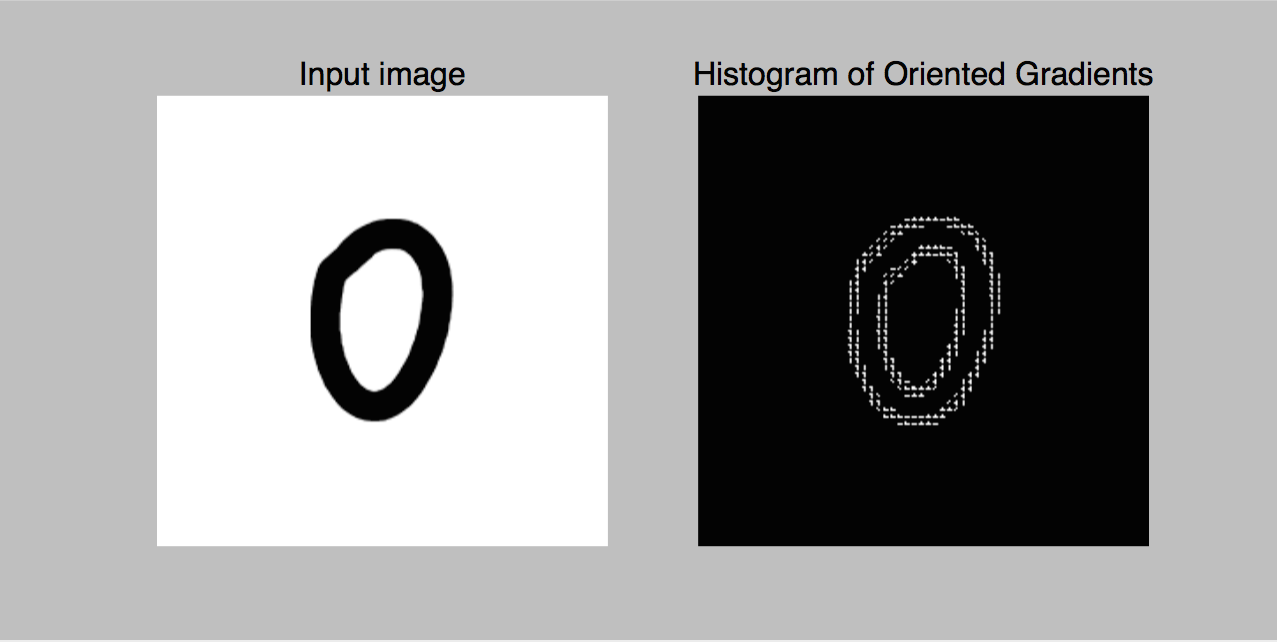
\includegraphics[width=\textwidth]{pictures/hog0}
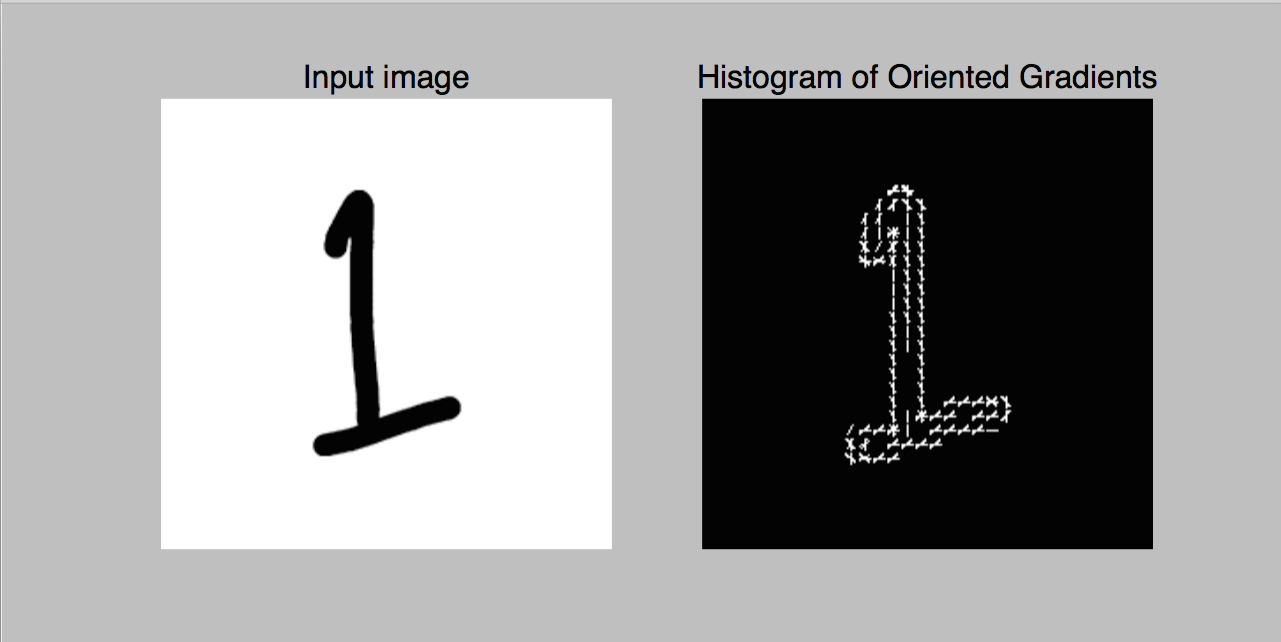
\includegraphics[width=\textwidth]{pictures/hog1}
\caption{Représentation du descripteur HOG pour les chiffres \emph{0} et \emph{1}}
\label{fig:hog}
\end{figure}

% ---------------------------------------
\section{Classification}

Pour classifier les chiffres, deux classifieurs différents ont été utilisés: un SVM et un réseau de neurones artificiels. Dans les deux cas, nous y avons ajouté une phase de grid-search avec cross-validation (k=10) lors de l'entrainement afin d'obtenir de bons jeux de paramètres. Les implémentations utilisées sont celles disponibles dans la librairie Python scikit-learn, car elles ont l'avantage justement d'offrir directement le grid-search et la cross-validation.

La figure \vref{fig:hog-svm-training} montre pour le SVM l'évolution du score en fonction du nombre d'exemple lors de la cross-validation.

\begin{figure}[!h]
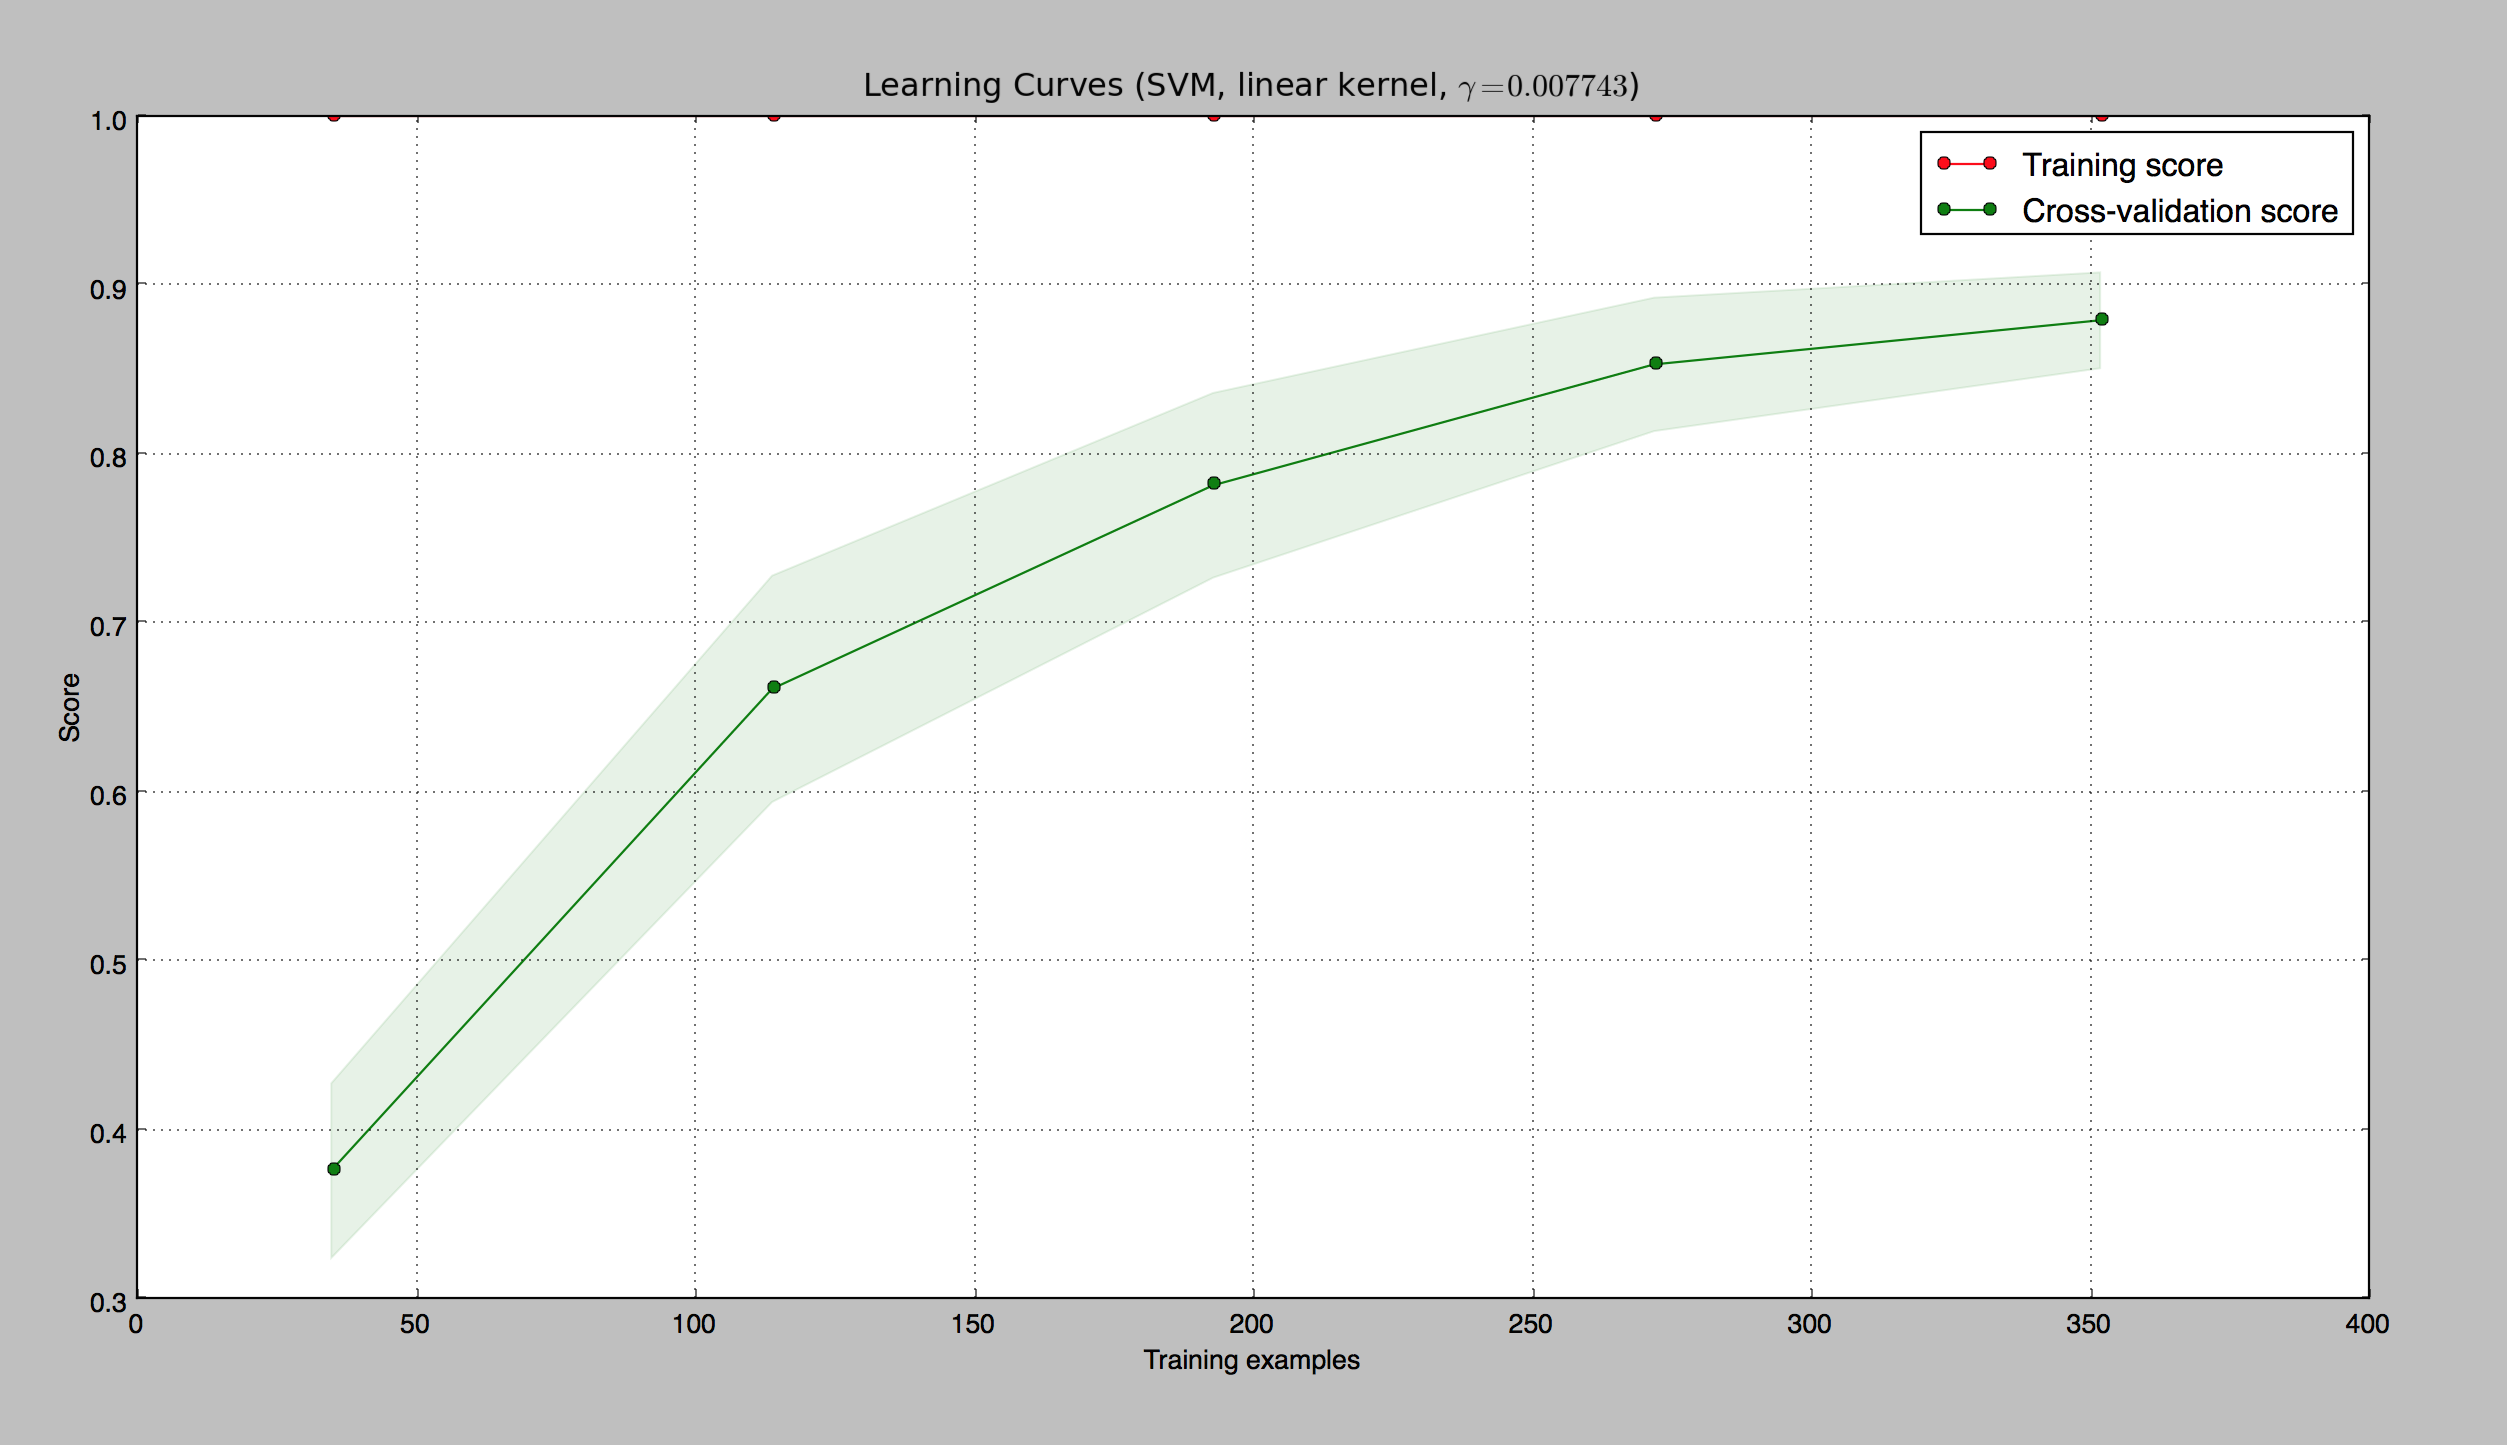
\includegraphics[width=\textwidth]{pictures/hog-svm-training}
\caption{SVM avec un noyau linéaire: Courbes d'apprentissage}
\label{fig:hog-svm-training}
\end{figure}

% ---------------------------------------
\section{Résultats}

Après exécution, nous avons obtenu les résultats suivants:
\begin{itemize}
\item SVM: 86\% de F1-score
\item Réseau de neurones: 93\% de F1-score
\end{itemize}
Nous constatons une différences de quelques pourcents entre les deux, toutefois cela peut s'expliquer par la différences du temps d'apprentissage des deux algorithmes: le grid-search du réseau de neurones a clairement été plus long que celui du SVM. Il est donc normal que les résultats puissent être meilleurs.

% ---------------------------------------
\section{Problèmes rencontrés}
Plusieurs problèmes ont été rencontrés:

\begin{itemize}
\item Utilisation excessives des ressources: lors des premières exécutions, nous avons constatés que le programme utilisait de plus en plus de ressources jusqu'à atteindre plus de 32 GB de RAM. Pour régler le problème, nous avons dû réduire la taille des images d'entrée et réduire le nombre de cellules pour le HOG.

\item Temps d'exécution important: les algorithmes ont dû tourner plusieurs jours avant de pouvoir obtenir les résultats du grid-search.

\end{itemize}

% ---------------------------------------
\section{Améliorations possibles}
Nous aurions voulu avoir un score pour 0-9a-z afin de pouvoir comparer les résultats avec ceux de SURF, mais par manque de temps nous n'avons pas pu l'obtenir.

\newpage
